% 导言区
\documentclass[a4paper,zihao=-4,linespread=1]{ctexrep}

\usepackage[]{animate}
\usepackage{color}
\usepackage{booktabs}
\usepackage{titlesec}
\usepackage{titletoc}
\usepackage[titletoc]{appendix}
\usepackage[normalem]{ulem}         % 关于下划线的一个宏包
\usepackage[]{indentfirst}          % 强制段首缩进
\usepackage[]{bm}
\usepackage[]{amsmath}
\usepackage[]{esint}
\usepackage[]{amssymb}
\usepackage[]{extarrows}
\usepackage{graphicx}
\usepackage[]{subfigure}
\usepackage[colorlinks,linkcolor=blue,bookmarksopen=true,bookmarksnumbered=true,citecolor=blue]{hyperref}             % 目录点击跳转
\usepackage[dvipsnames,svgnames]{xcolor}
\usepackage{tcolorbox}
\tcbuselibrary{breakable}   % 分页
\tcbuselibrary{skins}       % 箱子分页
\usepackage[]{tikz}
\usepackage[]{pgfplots}
\pgfplotsset{compat=1.18}
\usepackage{newtxtext}
\usepackage[strict]{changepage} % 提供一个 adjustwidth 环境
\usepackage{framed}             % 实现方框效果
\usetikzlibrary{positioning}   % tikz绘图相对位置
\tikzset{elegant/.style={smooth,thick,samples=50,cyan}}

% 定义公式环境
\newenvironment{lequation}{\large\begin{equation}}{\end{equation}}
\newenvironment{sequation}{\small\begin{equation}}{\end{equation}}
\newenvironment{tequation}{\tiny\begin{equation}}{\end{equation}}
% 定义方框
% 陈述性语句
\newtcolorbox[]{proposition}[2][]{title = \textbf{#2}, colback=Salmon!20, colframe=Salmon!90!Black,breakable, enhanced jigsaw}
% 历史注记
\newtcolorbox[]{history}[2][]{title = \textbf{#2}, colback=Emerald!10, colframe=cyan!40!black,breakable, enhanced jigsaw}
% 定理
\newtcolorbox[]{theorem}[2][]{title=\textbf{#2}, colback=red!5,colframe=red!75!black,breakable, enhanced jigsaw}
% 定义
\newtcolorbox[]{define}[2][]{title=\textbf{#2},colback=SeaGreen!10!CornflowerBlue!10,colframe=RoyalPurple!55!Aquamarine!100!,breakable, enhanced jigsaw}
% 思考注记
\definecolor{formalshade}{rgb}{0.99,0.97,0.93} % 文本框颜色
\newenvironment{thinknote}{%
\def\FrameCommand{%
\hspace{1pt}%
{\color{BurlyWood}\vrule width 2pt}%
{\color{formalshade}\vrule width 4pt}%
\colorbox{formalshade}%
}%
\MakeFramed{\advance\hsize-\width\FrameRestore}%
\noindent\hspace{-4.55pt}% disable indenting first paragraph
\begin{adjustwidth}{}{7pt}%
\vspace{2pt}\vspace{2pt}%
}
{%
\vspace{2pt}\end{adjustwidth}\endMakeFramed%
}

\setlength{\parindent}{4em}
\title{Notes of Griffiths Introduction to QM}   % 添加标题
\author{郑卜凡}                     % 添加作者
\date{\today}                             %最后更新日期

\begin{document}
    \maketitle              %制作封面
    \tableofcontents        %制作目录
    \setcounter{page}{0}
    \thispagestyle{empty}
    \chapter{波函数}
    \section{薛定谔方程}
    \begin{lequation}\label{S-1-D}
        \boxed{
            i\hbar\frac{\partial \Psi\left(x,t\right)}{\partial t}=-\frac{\hbar^{2}}{2m}\frac{\partial^{2}\Psi\left(x,t\right)}{\partial x^{2}}+
            V\left(x,t\right)\Psi\left(x,t\right)
        }
    \end{lequation}
    \begin{lequation}\label{S-3-D}
        \boxed{
            i\hbar\frac{\partial \Psi\left(\bm{r},t\right)}{\partial t}=\left[-\frac{\hbar^{2}}{2m}\nabla^{2}+
            V\left(\bm{r},t\right)\right]\Psi\left(\bm{r},t\right) 
        }
    \end{lequation}


    上面给出的公式中第一个是一维形式, 第二个是三维一般形式。对于某些公式推导上, 使用薛定谔方程时, 常常是对方程两边进行共轭操作\footnote[1]{物理实质可以理解
    为时间反演对称性}(以一维形式为例)也即:
    \begin{lequation}
        -i\hbar\frac{\partial \Psi^{*}\left(x,t\right)}{\partial t}=-\frac{\hbar^{2}}{2m}\frac{\partial^{2}\Psi^{*}\left(x,t\right)}{\partial x^{2}}+
        V\left(x,t\right)\Psi^{*}\left(x,t\right)
    \end{lequation}


    注意到上式的导出我们假定势能函数是实变函数, 这是有道理的, 但是书后面的习题\footnote[2]{详见第三版Problem1.17}也给出了一个例子, 那就是在不稳定的系统中, 找到粒子的概率不是守恒的, 也就是说$P$依赖于时间。
    这时如果引入含有虚部项的势能就可以很好地解释这一点。在量子力学中Schr{\"o}dinger方程的地位和牛顿第二定律一样, 现在只是描述粒子位置的函数变成了波函数。


    Born后面给波函数一个统计上的解释, 这也就说明了在量子力学中的不确定性, 我们无法再像牛顿运动定律一样精确的预言一个例子之后的运动, 我们只能给出它之后在某处的\uwave{概率}是多少
    \begin{proposition}{波函数的统计诠释}
        以一维情形为例, Born在统计上给出了对于波函数的解释, 他认为当一个微观粒子处于状态$Psi\left(\bm{r},t\right)$时, 表示在$t$时刻在$x$处发现粒子的\uwave{概率}, 更准确的说\footnote[0]{一个常用的代换是$\left|\Psi\left(x,t\right)\right|^{2}=
        \Psi^{*}\left(\left(x,t\right)\right) \Psi\left(x,t\right) $}
        \begin{lequation}
            \int_{a}^{b}\left|\Psi\left(x,t\right)\right|^{2}dx=\left\{\text{$t$时刻在$\left[a,b\right]$内\\发现粒子的概率}\right\}
        \end{lequation}
    
    \end{proposition}
    自然的, 我们会问, 测量时我们会发现粒子处于某点(C点), 那么测量之前粒子在哪?历史上有三种观点
    \begin{history}{测量前粒子在哪?}
        \textbf{1.现实主义学派:粒子还是在C点}, 这种观点完全否定了量子理论的不确定性, 也是爱因斯坦一直坚信的观点;\\
        \textbf{2.正统学派:粒子哪也不在}, 这种观点认为正是我们的测量\uwave{迫使}粒子在C点, 这个观点被广泛接受, 但到底什么是测量还有待讨论;\\
        \textbf{3.不可知论学派:拒绝回答}, 这种观点认为\uwave{测量前}本身就是难以定义的, 去讨论测量前粒子的位置也是没有意义的。
    \end{history}
    现代量子理论在实验上说明了正统学派的正确性\footnote[1]{John Bell在1964年派排除了不可知论}, 有一点需要注意, 测量会导致波函数的坍塌(\ref{fig-1.1}), 坍塌成了一个类似于狄拉克delta函数的图像, 在波函数还没有按照薛定谔方程重新弥散开来的时候继续测量, 我们会发现测量结果不变, 也
    就是说\uwave{测量完全改变了波函数}, 导致连续的测量得到的结果是一样的。

    既然波函数在统计上可以解释为概率密度分布函数, 那么一定要满足\textbf{归一化条件}
    \begin{proposition}{波函数归一化条件}
        \begin{lequation}\label{normalized}
            \int_{-\infty}^{\infty}\left|\Psi\left(x,t\right)\right|^{2}dx=1
        \end{lequation}
    \end{proposition}
    而且从薛定谔方程的线性性可以看出, 如果$\Psi$是方程的解, 那么$A\Psi$也一定是方程的解, 这里的A就类似于微分方程通解里面的系数, 你需要使用归一化条件去确定它, 求解出来的$A$是不需要考虑相位问题的, 不会在物理上产生任何影响, 你只需要确定
    它的模长就可以了, 下面一个关于归一化的定理让我们能更简单的对波函数进行归一化。
    \begin{theorem}{$A$是一个与时间无关的常数}
        \begin{lequation}
            \label{normalized-independent-time}
            \frac{d}{dt}\int_{-\infty}^{\infty}\left|\Psi\left(x,t\right)\right|^{2}dx=0
        \end{lequation}
    \end{theorem}
    由于这个定理的正确性, 我们找到波函数的一个可能解后, 只需要任意代入一个$t$的值, 然后将波函数乘上一个常数因子$A$对波函数进行全空间积分解出$A$的大小即得到了波函数的真正有物理意义的解, \textbf{任何无法进行归一化的解(比如$\Psi=0$)都要舍去}。
    \section{力学量的期望值和标准差}
    \begin{define}{数学上的定义: 平均值和标准差}
        \begin{center}
        \begin{math}
            \displaystyle
            \left \langle x \right \rangle \overset{\text{def}}{=}\int_{-\infty}^{\infty}x\rho(x)dx \qquad\qquad\qquad
            \sigma _{x}\overset{\text{def}}{=}\int_{-\infty }^{\infty } (x-\left \langle x \right \rangle )^2\rho(x)dx
        \end{math}
        \end{center}
        其中$\rho(x)$是概率密度函数, 把上面的$x$换成$f(x)$就可以得到某个一般量的平均值和标准差
    \end{define}
    根据上面的定义我们可以得到一个更加常用的计算标准差的公式: $\sigma(x)=\sqrt{\left \langle x^2 \right \rangle-\left \langle x \right \rangle^2}$。
    
    在进一步说明力学量的平均值的时候要先明确平均值的意义, 就比如说发现粒子所处位置的平均值, 你不能将其理解成连续测量一个系统很多次之后计算得到的平均值, 因为前面就说过
    波函数会由于测量而坍缩, 连续多次对一个系统的测量得到的结果是一致的! 这里对平均值的定义是对于\uwave{系综}的, 也就是你需要对大量相同状态下的系统进行测量来求平均值, 或
    者简单一点, 对一个系统测量很多次, 但每次测量要隔一段时间要等待波函数重新回到测量前未坍缩的样子。
    \begin{proposition}{位置和动量的算符}
        \begin{center}
            \begin{math}
                \displaystyle
                \hat{x}=[x] \qquad\qquad\qquad\qquad \hat{p}=\left[-i\hbar\frac{\partial}{\partial x}\right]    
            \end{math}
        \end{center}
        值得一提的是, 上面的动量算符是利用$\left \langle p \right \rangle=\frac{d\left \langle x \right \rangle}{dt}$得出来的
        \footnote[0]{这里的$\left \langle x \right \rangle$必须要事先写成关于$t$的函数, 另见Problem1.16(c)}
    \end{proposition}
    \begin{theorem}{任意一个力学量的统计量}
        \begin{lequation}
            \left \langle Q\left(x,p\right) \right \rangle=\int \Psi^{*}\left[Q\left(x,-i\hbar\frac{\partial}{\partial x}\right)\right]\Psi dx
        \end{lequation}
        \begin{equation}
            \sigma_Q = \sqrt{\left \langle Q^2 \right \rangle-\left \langle Q \right \rangle^2}
        \end{equation}
    \end{theorem}
    上面的定理说明了在量子力学中\uwave{算符}显得尤为重要, 你要计算一个力学量$Q$的平均值只要把这个力学量的算子\uwave{夹在}波函数中间再积分即可。确定一个力学量的算子时, 先将
    这个力学量由经典力学的公式表示成关于位置$x$和动量$p$的函数然后将$x$和$p$全部换成对应的算符即可。\footnote[1]{我们提倡使用算符这个新的工具去计算, 但有时候你会发现, 得到了$\left \langle x \right \rangle(t) $后直接使用
    $\left \langle p \right \rangle=\frac{d\left \langle x \right \rangle}{dx}$更快。有时候直接使用定义(波函数是实质是测量到粒子在位置$x$的概率密度分布函数), 用$\int x\left| \Psi(x,t)\right|dx$直接计算也能达到事半功倍
    的效果}
    \section{海森堡不确定性原理}
    这个原理在历史上曾经被称作\uwave{测不准原理}, 有很大的误导性, 实际上这个原理与测量误差毫无关系, 这是一个量子力学本身决定的原理。它表明了你对系统位置了解的越多, 比如说你把系统限制在某个
    确定的轨道狭槽内, 那么你对系统动量的了解程度一定越低, 测出来的动量分布肯定越是分散。其中动量与波函数之间的关系最早由德布罗意(de Broglie)给出:
    \begin{center}
    \begin{math}
        \displaystyle
        \boxed{
            p=\frac{h}{\lambda}=\frac{2\pi\hbar}{\lambda}
        }
    \end{math}
    \end{center}
    \begin{theorem}{Heisenberg Uncertainty Principle}
        \begin{lequation}
            \sigma_x\sigma_p \geq \frac{\hbar}{2} 
        \end{lequation}
    \end{theorem}
    \newpage
    \begin{figure}[htbp]
        \label{fig-1.1}
        \begin{tikzpicture}[scale=0.4] %缩放,还可以设置xscale, yscale
        \draw[->](4,-2)--(4,8) node[above]{$\Psi (x,0^-)$};
        \draw[->](0,2)--(12,2) node[below]{$x$};  % 画坐标轴
        \draw (4,2) node[below right]{$O$};
        \draw[elegant,domain=0:12] plot(\x,{5.5*exp(-(\x-6)^2/4.56)+2});
        \draw[dashed,red] (8,2)--(8,8);
        \draw (8,2) node[below]{$C$};
        \end{tikzpicture}  
        \hspace{4em}
        \begin{tikzpicture}[scale=0.4] %缩放,还可以设置xscale, yscale
        \draw[->](4,-2)--(4,8) node[above]{$\Psi (x,0^+)$};
        \draw[->](0,2)--(12,2) node[below]{$x$};  % 画坐标轴
        \draw (4,2) node[below right]{$O$};
        \draw[dashed,red] (8,2)--(8,8);
        \draw (8,2) node[below]{$C$};
        \draw[->,red] (8,2)--(8,6);
        \draw (8,6) node[right]{$\infty$};
        \end{tikzpicture}  
        \caption{在$t=0$时刻测量, 波函数将在$C$处坍塌为狄拉克$\delta$函数}
    \end{figure}
    \newpage
    \chapter{定态Schr\"{o}dinger方程}
    \section{定态和分离变量法}
    列出Sch\"{o}dinger方程后的下一步就是解出系统对应的波函数, 首先我们应该从最最初等的分离变量法来解方程, 毫无疑问我们只能通过它来\uwave{猜出}解空间
    的一小部分子集, 但是这种方法得出来的解却具有非常重要的物理意义, 后面的一系列讨论都默认势能函数不随时间变化(保守场)。

    分离变量法的基本思想就是将$\Psi$拆分为两个函数, 一个只关于$x$, 一个只关于$t$, 即$\Psi(x,t)=\psi(x)\phi(t)$, 带入到Sch\"{o}dinger方程(\ref{S-1-D})我们可以得到
    下面的式子\footnote[1]{$\phi(t)$附带的常数项我们合并到$\psi(x)$里面了,反正最后是对$\Psi$进行归一化}。
    \begin{lequation}
        \label{wiggle-function}
        \boxed{
            \phi(t)=e^{-\frac{iEt}{\hbar}}
        }
    \end{lequation}
    \begin{lequation}
        \label{time-independent-equation}
        \boxed{
            -\frac{\hbar^2}{2m}\frac{d^2\psi(x)}{dx^2}+V(x)\psi(x)=E\psi(x)
        }
    \end{lequation}

    式\ref{wiggle-function}你可以称之为\uwave{wiggle-function}, 它只和时间相关而且你如果使用Euler公式\footnote[2]{$e^{i\theta}=\cos\theta+i\sin\theta$}, 你
    会发现它是按照正弦规律进行\uwave{振动}的, 暂且就先把它当成是波函数里面的振荡项。后面的式子(\ref{time-independent-equation})及其重要, 它就是我们要
    谈的\textbf{定态薛定谔方程}, 不含时间, 其中的$E$实际上代表着系统的能量(哈密顿量\footnote[3]{哈密顿量就是动能加势能, 与系统的拉格朗日量对应, 后者是动能减势能})。
    \begin{define}{哈密顿算子}
        \begin{center}
           \begin{math}
            \displaystyle
            \hat{H}=\frac{\hat{p}^2}{2m}+[V]=-\frac{\hbar^2}{2m}\frac{\partial^2}{\partial x^2}+V
        \end{math} 
        \end{center}
    \end{define}
    使用哈密顿算子可以简化方程的书写为$\hat{H}\psi=E\psi$。下面列出来这些定态解重要的性质。
    \begin{theorem}{定态解$\Psi(x,t)=\psi(x)e^{iEt/\hbar}$}
        定态薛定谔方程的每个解都对应某个能量为$E$的\uwave{定态系统}:\\
        1.每个定态解对应系统能量(Hamiltonian)无论何时测量都是$E$,很容易通过证明它的方差和平均值都不随时变来证明它, 其它力学量的平均值也不随时变;\\
        2.定态解的时间项对概率密度没有任何贡献, i.e.用$\psi$替代$\Psi$去计算物理量的平均值不会产生任何差异, 因此有时候也刻意不区分两者;\\
        3.由于定态解能量的选取是任意的\footnote{实际上不完全任意}, 所以存在无穷多个定态解, 一般的解就是这些由分离变量得出来的定态解的\uwave{线性组合}
        \begin{lequation}
            \label{find_c}
            \boxed{
                \Psi(x,t)=\sum_{n=1}^{\infty}c_n\psi_n e^{-iE_nt/\hbar}
            }
        \end{lequation}
        其中常数$c$\footnote{可以是复数}需要使用初始波函数去确定。\\
        特别注意, 现在由定态解合成的一般解\textbf{不一定}是定态的, 而且比较遗憾的是一般你不能把它写成一个闭公式, 只能用无穷级数表示。
    \end{theorem}
    由于波函数需要满足归一化条件(eq.\ref{normalized}), 所以所有不满足归一化条件的解我们都应舍去, 他们是没有物理意义的, 所以这一步可以帮我们排除很多定态解
    的可能性。
    \begin{thinknote}
        这里实际上定态并不是我们真正要求的解, 我们要求的解是这些解的线性组合, 但是我们还是要将他们($\psi$)进行归一化处理, 但没有关系, 反正归一化只是乘上
        一个常数, 但在这里我们进行归一化后可以使得解的物理意义更加明朗, 更重要的是它会简化我们后续的数学对解的性质上的讨论。
    \end{thinknote}
    \begin{proposition}{定态解可归一化必要条件}
        1.能量$E$的虚部为零, 是一个实数;\\
        2.能量$E$要大于$V(x)$的最小值, 也就是说的能量不能一直小于势能\footnote{这个蛮好理解的, 因为动能项始终非负}。
    \end{proposition}
    \begin{proposition}{$c_n$的物理意义}
        一般解前面对于定态解$\Psi_n(x,t)=\psi(x)e^{-iE_nt/\hbar}$的权重$\left|c_n\right|^2$表示\textbf{测量到系统能量值为$E_n$的概率}, 这也意味着, 你
        对一个系统进行测量, 只可能得到它所包含的定态解分量对应的能量值, 一定是一组离散的值。
    \end{proposition}
    自然的, $c_n$也要满足归一化条件(eq.\ref{normalized-c})。注意, 我们上面提到是说在某次测量时发现系统能量为$E_n$, 而不是说系统在测量时处于能量为$E_n$的
    一个定态, 系统的态始终是没有发生改变的。而且我们也注意到系统的能量并不是一成不变的, 不同的测量显现出来的能量也不同, 但是系统的能量的平均值是随时间或者测量改变
    的(eq.\ref{energy-conservation}), 这一个性质就是在微观量子效应下的\textbf{能量守恒定律}。
    \begin{lequation}
        \label{normalized-c}
        \sum_{n=1}^{\infty}\left|c_n\right|^2=1
    \end{lequation}
    \begin{lequation}
        \label{energy-conservation}
        \left \langle H \right \rangle=\sum_{n=1}^{\infty}\left|c_n\right|^2E_n 
        \Rightarrow \frac{\partial H}{\partial t}=0\footnote[1]{实际上你也完全可以使用更简单的方式去计算, 即$\left \langle H \right \rangle=\int \Psi(x,t)^*\hat{H}\Psi(x,t) dx$, 你可以直接代入$t=0$进一步
        简化运算, 因为这个性质保证了平均能量与时间无关。}
    \end{lequation}
    \section{一维无限深方势阱}
    \begin{define}{The Infinite Square Well}
        粒子如果处于无限深势阱中, 那么它的势能可以写成下面的这种形式:
        \begin{center}
            \begin{math}
            \displaystyle
            V(x) = \begin{cases}
                    0, &0\leq x \leq a\\
                    \infty, & \text{otherwise}
                    \end{cases}
            \end{math}
        \end{center}
        就像是在$x=0$和$x=a$处由两堵墙, 粒子被困在两堵墙之间, 然而在两堵墙之间它可以\uwave{自由移动}。
    \end{define} 
    首先我们来看一下边界条件, 显然, 在势阱之外$\Psi(x,t)\equiv 0$, 同样也应该有$\Psi(0,t)=\Psi(a,t)=0$。根据定态薛定谔方程(eq.\ref{time-independent-equation}), 我
    们要去求解的是一个分段函数形式给出的微分方程, 不妨分段去考虑它, $(0,a)$之外波函数恒等于$0$, 对于$(0,a)$那一部分, 势能为$0$, 定态薛定谔方程写成\footnote{注意到$E\leq0$时的解是平凡的或者不能归一化的}:
    \begin{lequation}
        \boxed{
            -\frac{\hbar^2}{2m}\frac{d^2\psi}{dx^2}=k^2\psi,\quad k=\frac{\sqrt{2mE}}{\hbar}
        }
    \end{lequation}
    \begin{thinknote}
        实际上这里的$k$从经典力学上看可以理解为\textbf{角波数}, $k=2\pi/\lambda\xlongequal[]{de-Broglie-eq.}p/\hbar$, 使用经典力学的观点来看,粒
        子的能量为$E$, 那么动量为$\sqrt{2mE}$。
    \end{thinknote}
    这就是一个自由振子的数学模型, 代入边界条件并且归一化可以得到:
    \begin{lequation}
        \boxed{
            \psi_n(x)=\sqrt{\frac{2}{a}}\sin\left(\frac{n \pi}{a}x\right),\quad k=\frac{n \pi}{a}
        }
    \end{lequation}
    \begin{lequation}
        \boxed{
            E_n=\frac{n^2\pi^2\hbar^2 }{2ma^2}
        }
    \end{lequation}
    其中\textbf{$n$是正整数}。计算的时候你会发现, 两个边界条件实际上不能完全确定微分方程解的两个常数项, 但是它却限制了$ka=n\pi(n=1,2,3,\ldots)$, 而$k$
    的值和能量是相关的, 所以这也就说明了\textbf{量子力学系统中的定态解始终只能取一系列离散数值}, 又考虑到系统的真实解是定态解的叠加, 而且每次测量系统的能量
    时都会返回某个定态解的能量, 这也就体现了量子力学中\textbf{能量的不连续性}, 真正确定另一个常数的条件是归一化条件\footnote[2]{回想一下对$\Psi$归一化等价于对$\psi$归一化}。

    完整写下定态的波函数应该为:
    \begin{lequation}
        \Psi(x,t)=\sqrt{\frac{2}{a}}\sin\left(\frac{n \pi}{a}x\right)e^{in^2\pi^2\hbar t/2ma^2}
    \end{lequation}
    
    $n=1$时我们称作\textbf{基态}, 其它的我们称为\textbf{激发态}。观察不同解在$t=0$时的波函数(fg.\ref{fig-2.1})我们可以发现, 这些定态本质上就是一系列\uwave{驻波}, 势阱的
    两个边界是它的两个波节。
    \begin{figure}[htbp]
        \centering
        \subfigure[$n=1$]{
            \begin{tikzpicture}[scale=0.6] %缩放,还可以设置xscale, yscale
            \draw[->](0,-3)--(0,3) node[above]{$\Psi (x,0)$};
            \draw[->](-2,0)--(8,0) node[below]{$x$};  % 画坐标轴
            \draw (0,0) node[below right]{$O$};
            \draw (6,0) node[below]{$a$};
            \draw[elegant,domain=0:6] plot(\x,{3*sin(\x*pi/6 r)});
            \draw[-,red] (-2,0)--(0,0);
            \draw[-,red] (6,0)--(8,0);
        \end{tikzpicture} 
        }
        \subfigure[$n=2$]{
            \begin{tikzpicture}[scale=0.6] %缩放,还可以设置xscale, yscale
            \draw[->](0,-3)--(0,3) node[above]{$\Psi (x,0)$};
            \draw[->](-2,0)--(8,0) node[below]{$x$};  % 画坐标轴
            \draw (0,0) node[below right]{$O$};
            \draw (6,0) node[below]{$a$};
            \draw[elegant,domain=0:6] plot(\x,{3*sin(2*\x*pi/6 r)});
            \draw[-,red] (-2,0)--(0,0);
            \draw[-,red] (6,0)--(8,0);
        \end{tikzpicture} 
        } 
        \subfigure[$n=3$]{
           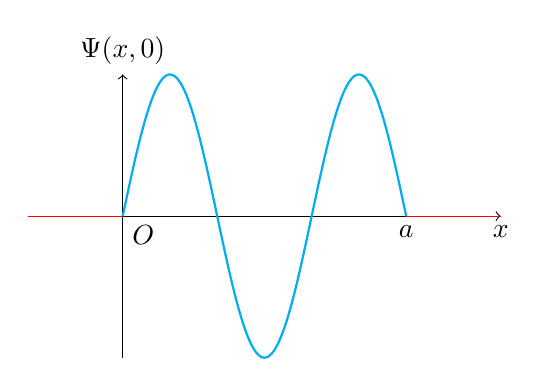
\begin{tikzpicture}[scale=0.6] %缩放,还可以设置xscale, yscale
            \draw[->](0,-3)--(0,3) node[above]{$\Psi (x,0)$};
            \draw[->](-2,0)--(8,0) node[below]{$x$};  % 画坐标轴
            \draw (0,0) node[below right]{$O$};
            \draw (6,0) node[below]{$a$};
            \draw[elegant,domain=0:6] plot(\x,{3*sin(3*\x*pi/6 r)});
            \draw[-,red] (-2,0)--(0,0);
            \draw[-,red] (6,0)--(8,0);
        \end{tikzpicture}   
        }
        \caption{不同的$n$对应不同的驻波波形}
        \label{fig-2.1}
    \end{figure}

    下面要谈到的性质虽然是根据无限深势阱总结来的, 但是他们却是普遍适用的\footnote[3]{$\delta$符号的相关定义见附录A}。
    \begin{theorem}{定态解的重要性质定理}
        1.不管势能本身是否具有对称性, 定态波函数总是关于势阱的中心成奇函数或偶函数(即关于中心轴对称或中心对称), 且随着$n$的变化交替出现;\\
        2.不管势能本身形状如何, 波函数的波节(零点)个数总是随着能量的增大而增大, 且公差为$1$;\\
        $\bigstar$3.\textbf{定态解之间相互正交}\footnote{回忆一下我们已经对$\psi$进行归一化}\footnote{积分为全空间, 对于无限深势阱积分限为$(0,a)$}
        \begin{lequation}
            \label{orthogonal}
            \int \psi_m(x)^*\psi_n(x) dx=\delta_{mn}
        \end{lequation} 
        $\bigstar$4.\textbf{定态解集合是完备的}:这个意思就是说你可以使用定态解的线性组合来表示\textbf{任何连续函数}, 对于这里的无限深势阱, 实质就是
        \uwave{傅里叶级数}。
    \end{theorem}
    上面的性质第四点说明了我们始终可以找到一组合适的$c_n$去满足初始波函数, 而如何去求这些$c_n$又是基于定态解的正交性(eq.\ref{orthogonal}), 使用傅里叶方法我们可以
    很容易的得到$c_n$\footnote[1]{$\Psi(x,0)$是初始波函数, 如果初始波函数不是在$t=0$时刻给定的, 你可能要额外考虑一下wiggle-function项(eq.\ref{wiggle-function})(更改时间原点也是一个不错的选择, 复习一下波动学里面的操作)}:
    \begin{lequation}
        \boxed{
            c_n=\int \psi_n(x)^*\Psi(x,0) dx
        }
    \end{lequation}

    使用正交性你还可以去证明\footnote[2]{分别基于初始波函数的归一化和定态薛定谔方程的算子表示法}eq.\ref{normalized-c}和eq.\ref{energy-conservation}。
    \begin{thinknote}
        上面的两个证明书上都有, 实际上你也可以证明按照上面的方法解出来的系统的波函数, $\Psi$已经自动归一化。但这是多此一举的, 因为无论是初始波函数, 还是确定$c_n$后的完整波函数, 波函数都是满足薛定谔方程的, 在
        前面的章节我们就说明了如果$\Psi$在某一时刻是归一化的, 那么之后任一时刻它也是归一化的(eq.\ref{normalized-independent-time})
    \end{thinknote}
    在计算能量平均值的级数时, 经常会涉及黎曼函数, 这里不做深入展开, 仅仅列出几个常用的和式。
    \begin{define}
        {黎曼$\zeta$函数}
        \begin{center}
            \begin{math}
                \displaystyle
                \zeta(s)\overset{def}{=}\frac{1}{1^s}+\frac{1}{2^s}+\frac{1}{3^s}+\frac{1}{4^s}+\cdots
            \end{math} 
        \end{center}
    \end{define}
    可以很容易的发现下面的等式成立:
    \begin{lequation}
        \boxed{
            \frac{1}{1^s}+\frac{1}{3^s}+\frac{1}{5^s}+\frac{1}{7^s}+\cdots = (2^s-1)\zeta(s)
        }
    \end{lequation}
    $s$为偶数时, 可以求出$\zeta$的精确值, 但对于奇数情况却异常复杂, 下面列出具体表达式和几个值供参考:
    \begin{theorem}{$s$为偶数时的解}
        \begin{center}
            \begin{math}
                \displaystyle
                \zeta(2n)=\eta_n \pi^{2n}
            \end{math}
            \begin{math}
                \displaystyle
                 \eta_1=\frac{1}{6},\qquad\eta_n=\sum_{k=1}^{n-1}(-1)^{n-1}\frac{\eta_{n-k}}{(2k+1)!} + (-1)^{n+1}\frac{n}{(2n+1)!}
            \end{math}
        \end{center}
    \end{theorem}

    \begin{table}[htbp]
        \centering
        \resizebox{\textwidth}{10mm}{
        \begin{tabular}{cccccccc} 
        \hline
        $s$     & $2$                & $4$                  & $6$                   & $8$                    & $10$                     & $12$                         & $14$                          \\ 
        \hline
        value & $\frac{\pi^2}{6}$ & $\frac{\pi^4}{90}$ & $\frac{\pi^6}{945}$ & $\frac{\pi^8}{9450}$ & $\frac{\pi^{10}}{93555}$ & $\frac{\pi^{12}}{638512875}$ & $\frac{2\pi^{14}}{18243225}$  \\
        \hline
        \end{tabular}}
    \end{table}

    \section{简谐振子}
    通过上一节我们已经大致知道了如何去求解特定势能下的波函数, 大致来说就是找到所有的定态解, 每一个解对应一个常量(能量), 这些常量的选取是离散的, 然后我们再
    对求出来的定态解进行叠加, 使用傅里叶方法定下权重即可。现在我们要碰到的势能函数形式是一个二次式, 但方程的求解却困难许多, 但这个工作是很有意义的, 因为任何
    势能函数的驻点附近, 使用Taylor展开, 你都可以将它处理成一个简谐振子的模型。
    \begin{define}{The Harmonic Oscillator}
        势能形式是关于$x$的二次式, 我们使用类似离心势能的形式写出:
        \begin{center}
            \begin{math}
                \displaystyle
                V(x)=\frac{1}{2}m\omega^2x^2
            \end{math}
        \end{center}
    \end{define}
    定态薛定谔方程相应的写成$$-\frac{\hbar^2}{2m}\frac{d^2\psi(x)}{dx^2}+\frac{1}{2}m\omega^2x^2\psi(x)=E\psi(x)$$
    这个方程可以使用幂级数解法去解决, 我们先介绍一种比较物理的方法去求解, 即\uwave{升降阶算符法}。
    \subsection{代数方法}
    \begin{define}{产生/湮灭算子}
        \begin{lequation}
            \hat{a}_\pm\overset{def}{=}\frac{1}{\sqrt{2m\omega\hbar}}(\mp i\hat{p}+m\omega x)
        \end{lequation}
    \end{define}
    \begin{thinknote}
        在计算算符时, 要格外小心, 算符一般情况下并不满足交换律, 你需要先将整个算符作用于一个函数上, 然后按照运算顺序逐个计算, 最后再进行化简。比如
        $x$和$\hat{p}$就不满足交换律\footnote[1]{量子力学很多与经典力学相冲突的地方就是因为这两个的不可交换性, 有的人将它当作公理去推导其它定理}, $
        x\hat{p}f(x)=-ix\hbar\frac{df}{dx}$但是$\hat{p}xf(x)=-i\hbar\frac{d}{dx}\left[xf(x)\right]=-i\hbar[f(x)+x\frac{df(x)}{dx}]$。
    \end{thinknote}
    \begin{define}{对易子}
        \begin{lequation}
            \left[\hat{A},\hat{B}\right]\overset{def}{=}\hat{A}\hat{B}-\hat{B}\hat{A}
        \end{lequation}
    \end{define}
    显然对易子是反对称的, 即$\left[\hat{A},\hat{B}\right]=-\left[\hat{B},\hat{A}\right]$, 计算可以得到下面很有用的关系式:
    \begin{lequation}
        \boxed{
            \left[x,\hat{p}\right]=i\hbar\qquad
            \left[\hat{a}_-,\hat{a}_+\right]=1
        }
    \end{lequation}
    第一个式子也常称作\textbf{正则对易关系}, 我们继续使用算子重写定态薛定谔方程:
    \begin{lequation}
        \boxed{
            \hat{H}=(\hat{a}_-\hat{a}_+-\frac{1}{2})\omega\hbar=(\hat{a}_+\hat{a}_-+\frac{1}{2})\omega\hbar
        }
    \end{lequation}
    \begin{lequation}
        \boxed{
            \omega\hbar(\hat{a}_+\hat{a}_-+\frac{1}{2})\psi(x)=E\psi(x)
        }
    \end{lequation}
    \begin{theorem}{谐振子的定态解}
        如果$\psi(x)$是谐振子在能量为$E$时的定态解, 那么$A\hat{a}_+\psi(x)$就是在能量为$E+\frac{1}{2}\omega\hbar$时的定态解\footnote[1]{前面乘上
        常数是归一化需要, 我们前面说过, 你求出来的解都需要进行归一化}, 同理, $A\hat{a}_-\psi(x)$是在能量为$E-\frac{1}{2}\omega\hbar$时的定态解。
    \end{theorem}
    直接根据湮灭和产生算子的定义可以很快地证明上述定理。现在很自然的就可以发现, 因为能量是不能一直递减的, 它至少要大于势能的最小值, 所以我们或许可以找到
    一个具有最低能量的定态解, 不能再使用湮灭算子产生新的解, 这个解我们称为$\psi_0(x)$, 是基态解。构造这个解的思路就是它的下一级是没有物理意义, 不能归一化的。
    也就是说有条件$$\hat{a}_-\psi_0(x)=0$$使用这个条件就可以得到基态解(不要忘了归一化)以及激发态解:
    \begin{lequation}
        \boxed{
            \psi_0(x)=\left(\frac{m\omega}{\pi\hbar}\right)^{\frac{1}{4}}e^{-\frac{m \omega}{2\hbar}x^2}
        }
    \end{lequation}
    \begin{lequation}
        \boxed{
            \psi_n(x)=\frac{1}{\sqrt{n!}}\left(\hat{a}_+\right)^n\psi_0(x),E_n=\left(n+\frac{1}{2}\right)\omega \hbar
        }
    \end{lequation}

    前面由归一化条件所决定的系数可以使用递推关系来确定, 再次强调, $\hat{a}_+\psi_n(x)=c_n\psi_{n+1}(x)$, $c$要根据归一化去确定, 并不是说使用产生算符可以
    直接得到高一个能级的解, 前面还有一个归一化条件确定的待定系数。
    \begin{theorem}{$\hat{a}_-$与$\hat{a}_+$是厄密共轭的(相互为伴随算子)}
        \begin{lequation}
            \int f^*(\hat{a}_\pm g)dx=\int (\hat{a}_\mp f)^* gdx
        \end{lequation}
    \end{theorem}
    直接计算$\left \| \hat{a}_+\psi_n(x) \right \|$和$\left \| \hat{a}_-\psi_n(x) \right \|$, 并利用$\hat{a}_+\hat{a}_-\psi_n=n\psi_n$及$\hat{a}_-\hat{a}_+\psi_n=(n+1)\psi_n$
    可以确定递推关系前面的系数(老规矩, 归一化只能确定模长, 但是我们只取最简单的那个值)。
    \begin{lequation}
        \boxed{
            \hat{a}_+\psi_n=\sqrt[]{n+1}\psi_{n+1},\quad\hat{a}_-\psi_n=\sqrt[]{n}\psi_{n-1}
        }
    \end{lequation}

    使用算符去表达可以使得计算更加简便, 你可以很容易的验证这些定态解之间相互正交, 所以可以使用傅里叶方法(你要求哪个常数, 你就在初态前面乘上对应的定态解, 然后
    全空间内积分, $t\neq0$时要考虑一下wiggle-function项)去定系数。计算力学量平均值的时候也可以使用产生湮灭算符去重新描述$x$和$\hat{p}$简化运算:
    \begin{lequation}
        \boxed{
            x =\sqrt[]{\frac{\hbar}{2m\omega}}\left(\hat{a}_++\hat{a}_-\right), \quad 
            p =i\,\sqrt[]{\frac{\hbar m \omega}{2}}\left(\hat{a}_+-\hat{a}_-\right)
        }
    \end{lequation}

    下面画出前三个能级对应波函数的能量, 不难看出图像具有的规律性和一维无限深势阱相同。
    \begin{figure}[htbp]
        \centering
        \subfigure[$n=1$]{
            \includegraphics[scale=0.7]{fig/2-3-a.eps}
        }
        \subfigure[$n=2$]{
            \includegraphics[scale=0.7]{fig/2-3-b.eps}
        }   
        \subfigure[$n=3$]{
            \includegraphics[scale=0.7]{fig/2-3-c.eps}
        }   
        \caption{可以看到, 图像之间的递推联系还是满足前面的规则的}
    \end{figure}
    \subsection{分析方法}
    \begin{define}{两个无量纲数}
        \begin{center}
            \begin{math}
            \displaystyle
            \xi = \sqrt{\frac{m\omega}{\hbar}}x \qquad\qquad K=\frac{2E}{\omega\hbar}
            \end{math}
        \end{center}
    \end{define}
    重写方程为:
    \begin{lequation}
        \label{rewrite}
        \frac{d^2\psi}{d\xi^2}=(\xi^2-K)\psi
    \end{lequation}
    \begin{thinknote}
        你可能对这个形式的得到有所疑问, 实际上, 这就是一个求导的链式法则的问题, 注意, 换元前的方程$\frac{d\psi}{dx}$表示把$\psi$写成$f(x)$后再求导, 而
        换元后的方程中$\frac{d\psi}{d\xi}$表示将$\psi$表示为$\phi(\xi)$后再进行求导。而$\xi=\varphi(x)$, 使用链式法则便可以理解这里的换元了。
    \end{thinknote}
    使用幂级数方法求解的第一步就是去求其\uwave{渐进解}, 也就是说去观察$\xi \to \pm\infty$的时候方程的行为。这个方程在$\xi\gg K$时
    $$\frac{d^2\psi}{d\xi^2}\approx\xi^2\psi$$这个方程的通解形式是$$\psi\approx Ae^{-\xi^2/2}+Be^{\xi^2/2}$$显然$B\neq 0$时波函数不能进行归一化, 所
    以, 方程\ref{rewrite}的解的形式应该是$\psi = h(\xi)e^{-\xi^2/2}$, 代入后有$$\frac{d^2h}{d\xi^2}-2\xi\frac{dh}{d\xi}+(K-1)h=0$$这是一个二阶方程
    但是是变系数, 所以也很难求解, 只能考虑使用幂级数解法, 两边进行Taylor展开后解得$$h(\xi)=\sum_{j=0}^\infty a_j\xi^j,\qquad a_{j+2}=\frac{2j+1-K}{(j+1)(j+2)}a_j$$
    我们只要确定$a_0$和$a_1$也就可以确定解, 二阶方程刚好两个待定系数, 但是我们只有波函数归一化这一个方程似乎无法去完整的确定两个待定系数。这里的原因是能量
    的量子化取值, 导致了最后方程只会含有一个待定系数。

    我们可以证明, $h(\xi)$只能在某些特定的情况下在$\xi \to \pm \infty$时收敛, 这也就决定了\textbf{$K$的取值是量子化的}。事实上, 收敛的充要条件是, 上面的数列$\{a_j\}$
    会终止于$0$。
    \begin{proposition}{$a_j$会终止于$0$}
        \begin{center}
            \begin{math}
            \displaystyle
            K=2n+1,\quad (n=0,1,2,\ldots)
            \end{math}
        \end{center}
        如果$n$是奇数, 那么$a_{2n+1}$会终止于$0$, 但是$a_0=0$也就是说必须有$a_{2n}\equiv 0$, $n$为偶数时类似
    \end{proposition}
    这样方程最终得到的解就只会有一个待定系数了, 而且由递推公式得知是正比于$a_0$或$a_1$的, 再利用归一化条件便可以得到解
    \begin{define}{厄米多项式}
        把$h(\xi)$的$a_0$或者$a_1$因子去掉并且乘上一个数将最高次项前面的因子化为$2^n$, 得到的多项式为\textbf{厄米多项式}, 记作$H_n(\xi)$\\
        例如:$h_2(\xi)=a_0(1-2\xi^2)=-\frac{1}{2}a_0(4\xi^2-2)$则$H_2(\xi)=4\xi^2-2$
    \end{define}
    我们不加证明地列出波函数归一化后的解与厄米多项式之间的关系\footnote[1]{前面因子的相位按照惯例按最简单的取}:
    \begin{lequation}
        \boxed{
            \psi(x)=\left(\frac{m\omega}{\pi\hbar}\right)^{\frac{1}{4}}\frac{1}{\sqrt{2^nn!}}H_n(\xi)e^{-\xi^2/2}
        }
    \end{lequation}
    \begin{theorem}{$H_n(\xi)$的诸多性质}
        \begin{itemize}
            \item 
                \begin{math}
                    \displaystyle
                    H_n(\xi)=(-1)^ne^{\xi^2}\left(\frac{d}{d\xi}\right)^ne^{-\xi^2}
                \end{math}
            \item 
                \begin{math}
                    \displaystyle
                    H_{n+1}(\xi)=2\xi H_n(\xi)-2nH_{n-1}(\xi)
                \end{math}
            \item 
                \begin{math}
                    \displaystyle
                    \frac{d H_n}{d\xi}=2n H_{n-1}(\xi)
                \end{math}
            \item 
                \begin{math}
                    \displaystyle
                    e^{-z^2+2z\xi}=\sum_{n=0}^{\infty}\frac{z^n}{n!}H_n(\xi)\quad\text{(generate function)}
                \end{math}
        \end{itemize}
    \end{theorem}
    量子效应下, 谐振子的行为和经典力学非常不同, 不再有\uwave{振幅}这一概念, 粒子可以在无穷远处被发现, 不违背能量守恒定律正是因为量子力学中, 我们只谈系综的
    力学量的平均值, 不再对于某个粒子有诸如动能这些的定义了, 我们只讲系综的平均效应, 只谈概率, 不谈确定性。
    \section{自由粒子}
    自由粒子情况下即$V \equiv 0$, 不难发现定态薛定谔方程和无限深势阱的形式是一样的, 即$$\frac{d^2\psi}{dx^2}=-k^2\psi$$解的形式为$$Ae^{ikx}+Be^{-ikx}$$
    注意, \uwave{我们不再有边界条件去直接确定$A$和$B$的值}, \textbf{这个时候定态解的能量的取值并不是离散的!可以取到任何大于$0$的值!}其实本身量子力学就是不排斥
    连续性的, 离散可以有很多种, 不一定就表明某个量一定是离散取值。

    考虑wiggle-function后写成下面的形式\footnote[1]{这里$\psi_k$无法进行归一化, 不像前面一样我们先进行归一化后再去定系数会有很多便利。但是这里我们还是在
    前面添了一个$\frac{1}{\sqrt{2\pi}}$你很快就可以看见他在数学处理上的妙处}:
    \begin{lequation}
        \boxed{
            \Psi_k(x,t)=Ae^{i\left(kx-\frac{k^2\hbar}{2m}\right)}, \psi(x)=\frac{1}{\sqrt{2\pi}}e^{ikx}
        }
    \end{lequation}
    考虑到最后反正要对解进行线性叠加, 而两项仅仅只在$e$指数上面差了一个负号, 所以我们将负号纳入$k$后得到:
    $$k\overset{def}{=}\pm\frac{\sqrt{2mE}}{\hbar}$$观察到每一项就代表一个\uwave{行波}, $k<0$的时候正向传播, 反之负向传播, 不再是前面势阱模型里面的
    驻波。
    
    与经典力学中的波动方程相对应, 前面讲过$k$可以理解为角波数, 那么波速$v=\frac{|k|\hbar}{2m}=\sqrt{\frac{E}{2m}}$, 角频率$\omega=\frac{k^2\hbar}{2m}$, 过会我们会再回到波速的问题上来, 目前
    来看似乎有自由粒子速度$v_p=\sqrt{\frac{2E}{m}}=2v_{wave}$。

    自由粒子的波函数的定态解与前面两个模型最大的不同就是\textbf{它是无法归一化的}。所以现在我们求出来的定态解完全只是数学上的一个过程, 没有实际的物理意义
    不存在一个状态, 其中自由粒子属于能量始终不变的定态(无论如何测量都是一个值)。但是没事, 虽然不存在定态, 但是我们还是可以使用定态解的线性组合来构造符合初值的
    解\footnote[2]{这些合成的解沿用波动学的观点, 称为\uwave{波包}, 是可归一化的}, 这些“定态”解也是归一化和完备的。

    我们仍旧对定态解进行线性叠加, 注意是对定态解叠加, 也就是对定态解的波函数进行叠加不是$\psi$而是$\Psi$, 所以不要忘记了每个$\psi$后面的关于时间的指数项。
    \begin{lequation}
        \boxed{
            \Psi=\int_{-\infty}^{\infty}\phi(k)\psi_ke^{-\frac{ik^2\hbar}{2m}}dk=\frac{1}{\sqrt{2\pi}}\int_{-\infty}^{\infty}\phi(k)e^{i\left(kx-\frac{ik^2\hbar}{2m}\right)}dk  
        }
    \end{lequation}
    和\ref{find_c}对比一下就会发现, $\phi(k)$取代了$c_n$, 这一点很好理解, 因为$\phi_k(x)$变成了一个关于$k$的连续函数, 而数列我们也通常称为\uwave{整标函数}, 所
    以, 前面变成连续函数来加权, 求和也变成了积分。

    初始值还是在$t=0$处给定\footnote[1]{若不是, 你对$t$进行一个换元平移一下计时零点即可}, 那么可以得到:
    \begin{lequation}
        \Psi(x,0)=\frac{1}{\sqrt{2\pi}}\int_{-\infty}^{\infty}\phi(k)e^{ikx}dk  
    \end{lequation}
    数学上$\Psi$就是对$\phi$的傅里叶变换, 下面的定理可以很方便的求出$\phi(k)$。
    \begin{theorem}{Plancherel's theorem}
        \begin{center}
            \begin{math}
                \displaystyle
                f(x)=\frac{1}{\sqrt{2\pi}} \int\limits_{-\infty}^{\infty}F(k)e^{ikx}dk\Longleftrightarrow F(k)=\frac{1}{\sqrt{2\pi}} \int\limits_{-\infty}^{\infty}f(x)e^{-ikx}dx
            \end{math}
        \end{center}
    \end{theorem}
    \begin{lequation}
        \boxed{
            \phi(k)=\frac{1}{\sqrt{2\pi}} \int _{-\infty}^{\infty}\Psi(x,0)e^{-ikx}dx
        }
    \end{lequation}
    
    遗憾的是, 很多函数都只能写出积分后进行数值模拟, 无法用基本初等函数表示。
    \begin{define}{群速度和相速度}
        \begin{itemize}
            \item \textbf{群速度}:波包的移动速度
            \item \textbf{相速度}:波包里面有很多小峰, 这些小峰的移动速度便是相速度, 可以理解为一个在波上的质点跟随波的平移速度
        \end{itemize}
    \end{define}
    \animategraphics[scale=0.75,autoplay=True,loop]{24}{videos/wave_group/wave_group-}{0}{250}
    \begin{center}
        上面的动画中, {\color{red}红色}表示相速度, {\color{green}绿色}表示群速度
    \end{center}
    
    关于群速度和相速度的讨论应该是波动学的内容, 这里我们不想讨论过多, 只是先说明两个速度的计算公式, 在波包很明显也就是有很好的群速度的定义的时候, 单单从
    自由粒子的波动方程可以推出下面这一点。
    \begin{theorem}{群速度和相速度的计算}
        \begin{lequation}
            \boxed{
               v_g=\frac{d\omega}{dk}\qquad\qquad v_p=\frac{\omega}{k} 
            }
        \end{lequation}
    \end{theorem}
    正是由于多列行波的叠加才形成了波包, 而每个分量(行波)中的频率又是和$k$相关的, 这样就会导致群速度不等于相速度, 这时我们称之为\textbf{色散}, 自由粒子的
    波函数恰好就是多列行波的叠加, $\omega$是关于$k$的二次式, 那么, 代表粒子的群速度是代表行波前进的相速度的两倍这一论断就不难看出了。
    \section{\texorpdfstring{$\delta$}.函数势阱}
    \titleformat{\chapter}[display]
{\normalfont\Large\bfseries}{Appendix~\Alph{chapter}}{11pt}{\Large}

\appendix
\renewcommand{\thechapter}{\Alph{chapter}}
\chapter{Vector Calculus}
\section{指标运算}
指标运算其实就是在涉及到向量, 张量求和表示时, 频繁的使用$\Sigma$会降低文章的可读性, 索性人为的\uwave{规定}去掉求和符号。
\begin{proposition}{爱因斯坦求和约定}
    只要是某一项中出现的两个相同的指标\footnote{$\bigstar$不可能在某一项中出现三个相同的指标。}, 那么就理解为对这个指标求和也就是说
    \begin{center}
        \begin{math}
            \displaystyle
            c_i = \sum_{j=1}^{3}a_{ij}b_{j} \Longleftrightarrow c_i=a_{ij}b_{j} \text{\quad} (i=1,2,3)
        \end{math}
    \end{center}
    我们称$j$为\uwave{哑指标},$i$为\uwave{自由指标}, 总的来说, 这就是一种方便使用的约定记号, 而且有时候去掉求和符号后能够是我们更加清晰地进行计算。
\end{proposition}
指标运算这个东西实际上非常微妙, 一方面它能帮助你大幅度的简化运算, 另一方面它的一些操作总是让人头晕。关于哑指标和自由指标, 你需要记住的就是哑指标只是
表示求和, 所以你可以更换字母或者对换字母, 例如:$a_ib_i=a_jb_j$, $a_{ij}b_{ji}=a_{ji}b_{ij}(i\leftrightarrow j)$, 而自由指标更像是在表示某个向量
的某一个分量, 你需要对等式两边同时去替换。
\begin{define}{符号定义}
    1.克罗内克符号(Kronecker delta)\qquad\qquad
    \begin{math}
        \centering
        \delta_{ij}=\begin{cases}
            0,& i \neq j\\
            1,& i=j
        \end{cases}
    \end{math}\\
    2.列维-奇维塔符号\footnote{$\tau$表示逆序数}(Levi-Civita symbol)\\
    \begin{center}
    \begin{math}
        \epsilon_{ijk}=\begin{cases}
            1,&\tau(ijk)\text{ is even}\\
            -1,&\tau(ijk)\text{ is odd}\\
            0,&\text{any of $i,j,k$ is equal}
        \end{cases}
    \end{math} 
    \end{center}
\end{define}    
克罗内克符号常常被用来\uwave{替换指标}, 下面的关系在简化运算时非常有用。
\begin{lequation}
    \boxed{
        \delta_{ij}a_j=a_i \qquad \qquad \delta_{ij}a_{jk}=a_{ik}
    }
\end{lequation}

也就是说一旦碰到相同的指标$\delta$会将那一项的这个指标替换为$\delta$的另一个指标, 比如上面的公式$\delta$作用为$j\leftrightarrow i$。

$\epsilon$和$delta$之间有一个十分有用的关系式:
\begin{lequation}
    \boxed{
        \epsilon_{ijk}\epsilon_{klm}=\delta_{il}\delta_{jm}-\delta_{im}\delta_{jl}
    }
\end{lequation}
\begin{thinknote}
    \textbf{几个使用求和约定表示的例子:}\\
    \begin{math}
        \displaystyle
        \bm{a}\cdot\bm{b}=a_ib_i \qquad\qquad [\bm{a}\times\bm{b}]_i=\epsilon_{ijk}a_jb_k\\
        \bm{A}\bm{B}_{ij}=\bm{A}_{ik}\bm{B}_{kj} \qquad\qquad \bm{A}^{T}_{ij}=\bm{A}_{ji}\\
        \left|\bm{M}\right| =\epsilon_{ijk}\bm{M}_{1i}\bm{M}_{2j}\bm{M}_{3k}\Longleftrightarrow \epsilon_{pqr}\left|\bm{M}\right|=\epsilon_{ijk}\bm{M}_{pi}\bm{M}_{qj}\bm{M}_{rk}
    \end{math}
\end{thinknote}
\section{梯度, 散度, 旋度}
\begin{define}{Gradient}
    \begin{enumerate} 
        \item  梯度可以定义为垂直于等值面的向量, 且模长等于势随等值面垂直距离的变化率
        \item  使用$df=\nabla f\cdot\bm{dr}$定义梯度($\nabla f \longleftrightarrow \bm{grad}f$)
        \item  \begin{math}
                \displaystyle
                \nabla f\overset{def}{=}\lim_{\delta V \to 0}\frac{1}{\delta V} \varoiint_{\delta S} f \bm{n}dS
                \end{math}
    \end{enumerate}
\end{define}
\begin{define}{Divergence}
    \begin{center}
        \begin{math}
        \displaystyle
        \nabla \cdot \bm{u} \overset{def}{=}\lim_{\delta V \to 0}\frac{1}{\delta V} \varoiint_{\delta S} \bm{u} \cdot \bm{n}dS
        \end{math}
    \end{center}
\end{define}
\begin{define}{curl}
    \begin{center}
        \begin{math}
        \displaystyle
        \nabla \times \bm{u} \cdot \bm{\hat{n}} \overset{def}{=}\lim_{\delta S \to 0}\frac{1}{\delta S} \oint_{\delta C} \bm{u} \cdot \bm{dr}
        \end{math}\footnote[0]{$\hat{n}$是垂直于$\delta S$面元的单位矢量, 且与曲线积分绕行方向遵循右手螺旋定则}
    \end{center}
\end{define}
在直角坐标系下, 这些量的表达式只要使用$\nabla\overset{def}{=}(\frac{\partial}{\partial x},\frac{\partial}{\partial y},\frac{\partial}{\partial z})$, 类比
为向量运算法则即可, 使用爱因斯坦求和约定可以进一步简化表达式, 并进行清晰的推演, 下面列举出来的是比较重要的矢量分析公式, 除了极个别公式, 都可以用求和约定快速
推导出来。
\begin{theorem}{一些矢量公式}
    \begin{itemize}
        \item $\nabla \cdot (\nabla f)=\nabla^2 f$\footnote[1]{也可以写为$\triangle f$定义为拉普拉斯算子}
        \item $\nabla \times (\nabla f)=0$
        \item $\nabla \cdot (\nabla \times \bm{u})=0$
        \item $\nabla \times (\nabla \times \bm{u})=\nabla(\nabla\cdot \bm{u})-\nabla^2\bm{u}$
        \item $\nabla (fg)=f\nabla g+g\nabla f$
        \item $\nabla \cdot (f\bm{u})=\nabla f \cdot \bm{u} + f\nabla\cdot \bm{u}$
        \item $\nabla \times (f\bm{u})=\nabla f \times \bm{u}+f\nabla\times\bm{u}$
        \item $\nabla \cdot (\bm{u}\times\bm{v})=(\nabla\times\bm{u})\cdot\bm{v}-(\nabla\times\bm{v})\cdot\bm{u}$
        \item $\nabla \times (\bm{u}\times\bm{v})=\bm{u}(\nabla\cdot\bm{v})+(\bm{v}\cdot\nabla)\bm{u}-(\bm{u}\cdot\nabla)\bm{v}-\bm{v}(\nabla\cdot\bm{u})$\footnote[2]{这里$\bm{u}\cdot\nabla\overset{def}{=}u_i\frac{\partial}{\partial x_i}$}
        \item $\nabla(\bm{u}\cdot\bm{v})=\bm{u}\times(\nabla\times\bm{v})+\bm{v}\times(\nabla\times\bm{u})+(\bm{u}\cdot\nabla)\bm{v}+(\bm{v}\cdot\nabla)\bm{u}$
    \end{itemize}
\end{theorem}
除了这些公式, 使用梯度、散度和旋度的相关定理可以推导出关于积分的重要公式, 在这些公式中取某些特殊情况可以得到其它实用的公式(格林公式):
\begin{theorem}{Gauss 定理}
    \begin{center}
       \begin{math}
            \displaystyle
            \iiint_V \nabla \cdot \bm{u} dV=\varoiint_S \bm{u} \cdot\bm{dS}
        \end{math} 
    \end{center}
\end{theorem}
\begin{theorem}{Stokes 定理}
    \begin{center}
        \begin{math}
            \displaystyle
            \iint_S \nabla \times \bm{u}\cdot\bm{dS}=\oint_C \bm{u}\cdot\bm{dr}
        \end{math}
    \end{center}
\end{theorem}
上面两个定理给了你一个途径, 将积分式转化为微分式, 比如Maxwell方程组的两种形式转化, 还有电解质里面的极化电荷体密度和极化强度之间的关系。
其它关于格林公式等公式的导出从略, 主要思路就是选取特殊的积分向量函数你还可以根据高斯定理结合量的守恒定律推出连续性方程:
\begin{lequation}
    \boxed{
        \frac{\partial \rho}{\partial t}+\bm{u}\cdot\nabla\rho+\rho\nabla\cdot\bm{u}=0
    }
\end{lequation}
\section{曲线坐标系}
实际上要在空间中确定点的坐标, 我们真正意义上是使用的叫做\textbf{坐标曲线}的东西来确定的。比如$u_1(x,y)=c_1$你就可以看作是一个坐标曲线, 不同的方程右边不同的常数值
也就对应了不同的曲线, 再取一个曲线簇$u_2(x,y)=c_2$, 这些曲线簇会有无限多个交点, 布满整个坐标平面, 那么我们就可以使用$(c_1,c_2)$来表示一个交点的坐标, 就是告诉你
是哪条曲线和哪条曲线相交。比如说经纬度就是这个样子, 用经线和纬线的交点来确定位置。常见的直角坐标系可以看作是$x=c_1$, $y=c_2$的特例, 这个定义也可以自然的推广到三维去, 只
是这个时候坐标曲面取代了坐标曲线, 两个坐标曲面的交点再被定义成坐标曲线。
\begin{figure}[htbp]
    \centering
    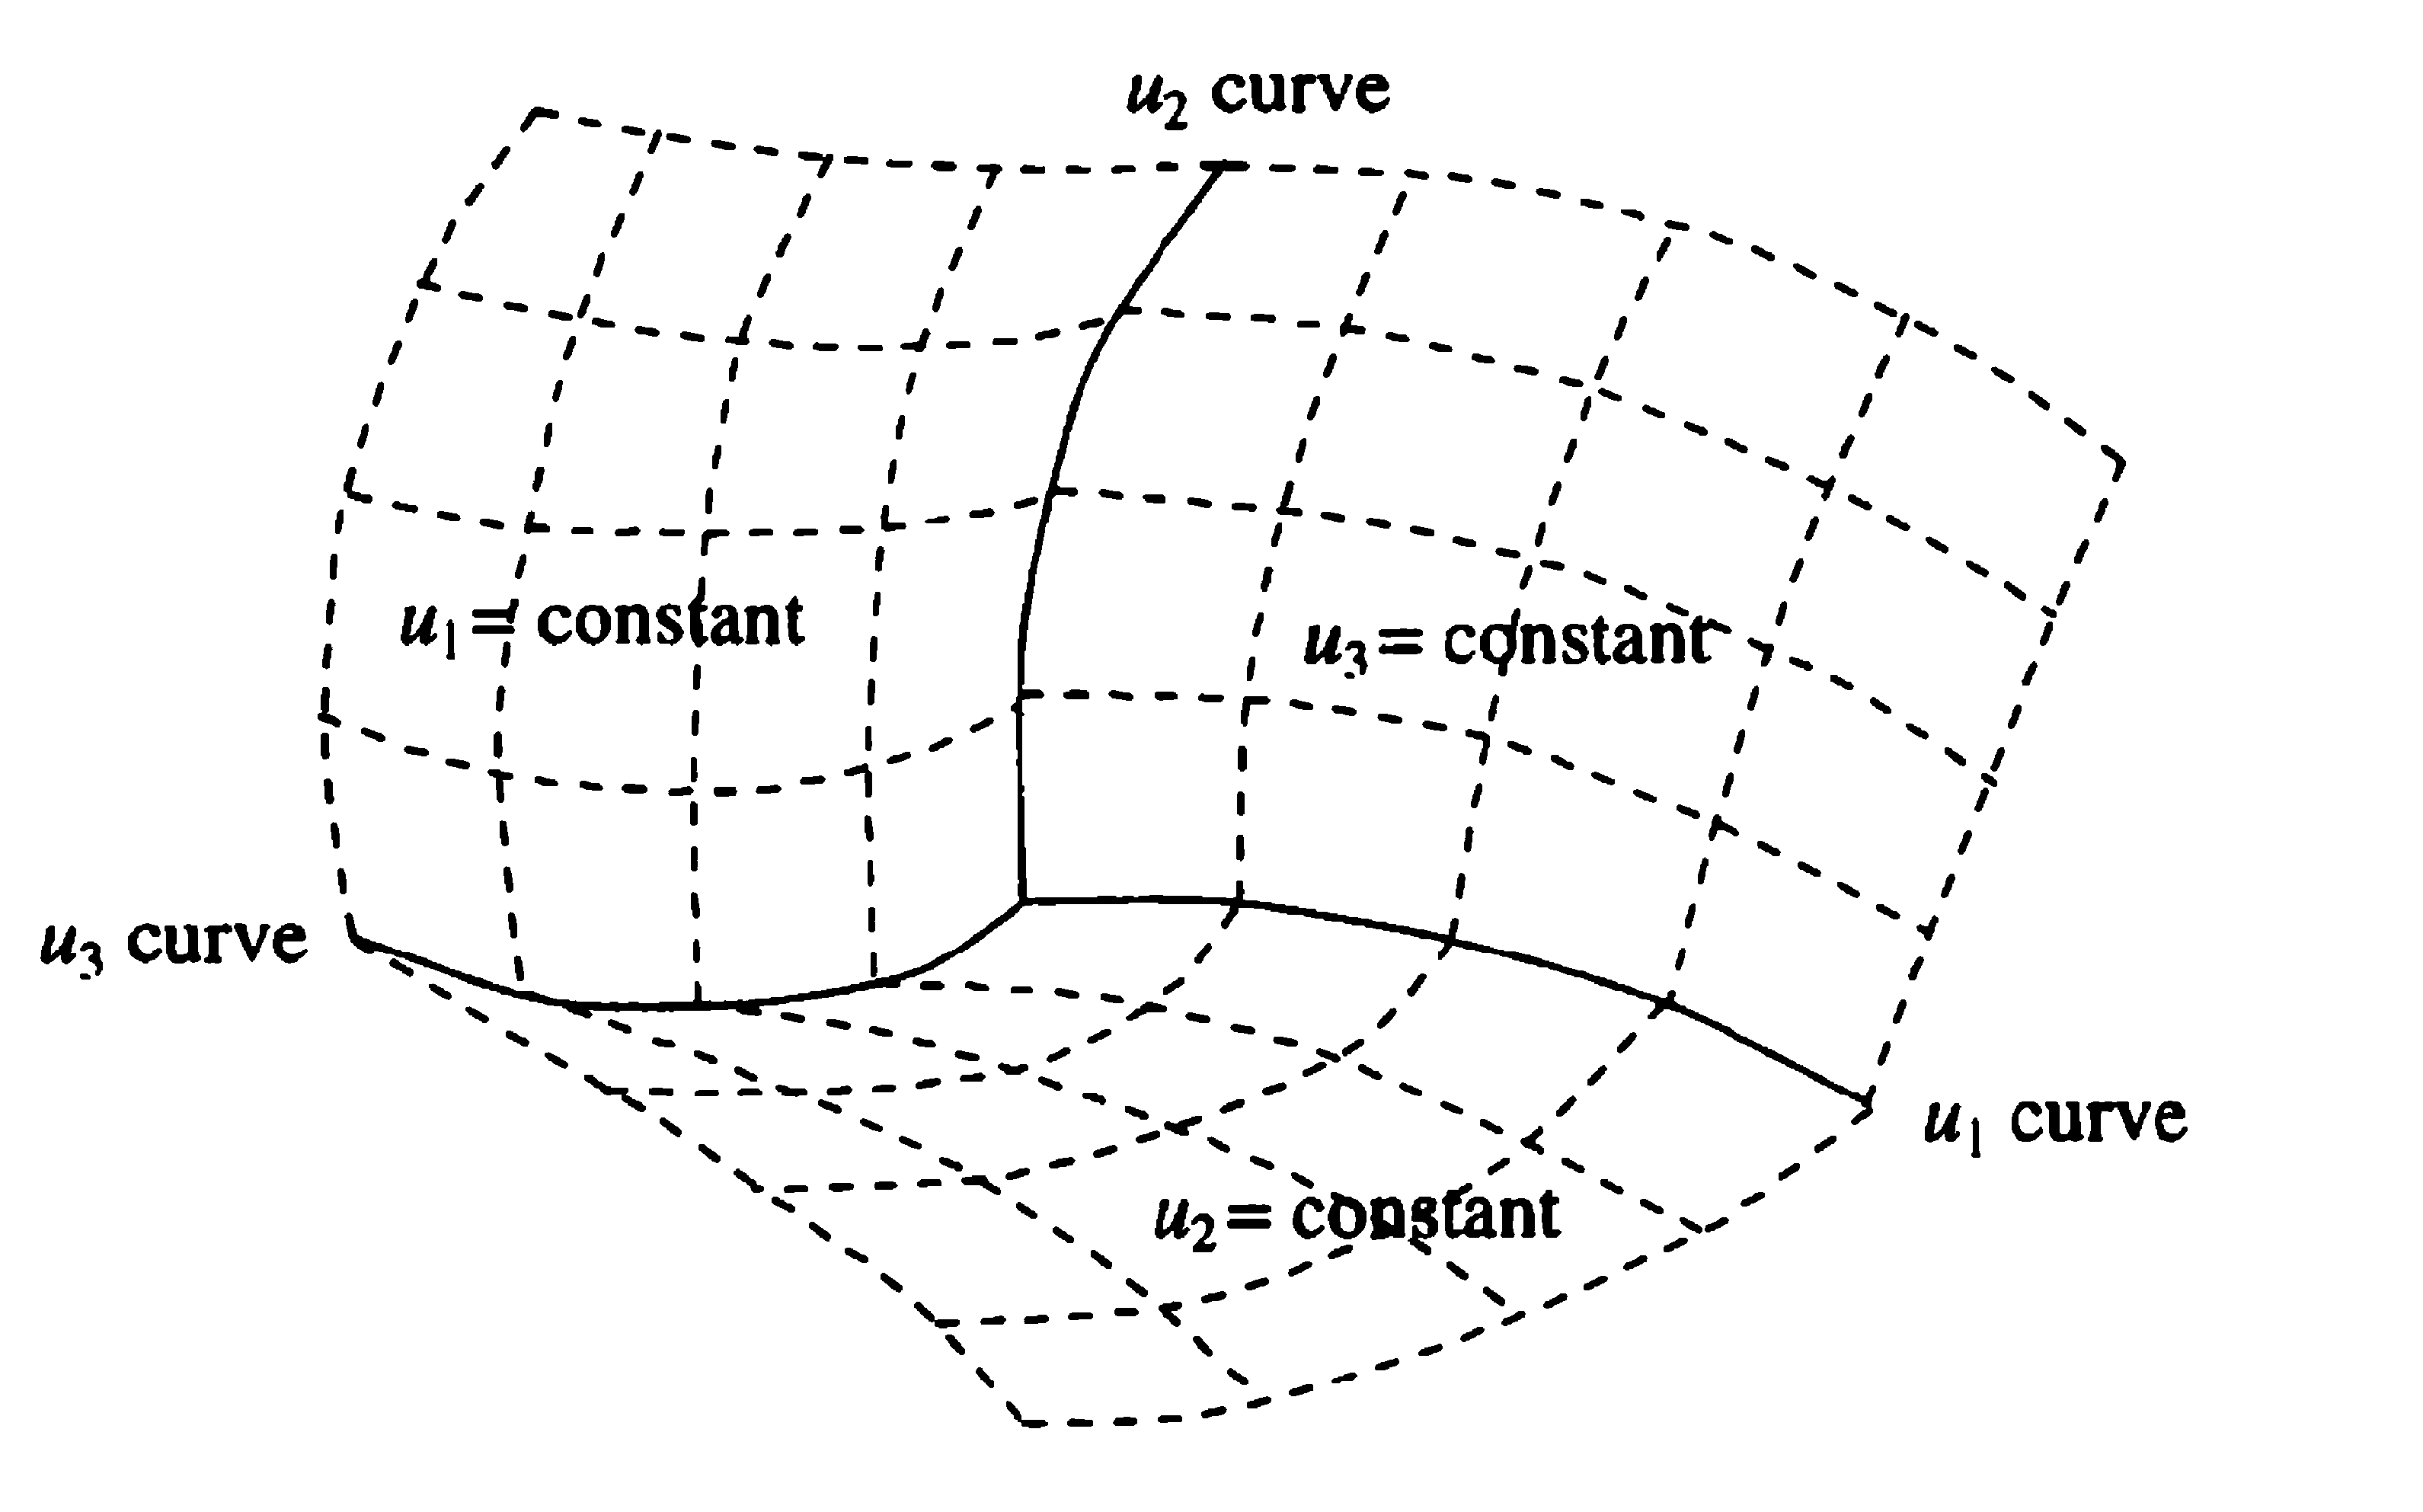
\includegraphics[scale=0.26]{fig/a-1.eps}
    \caption{曲线坐标系}
\end{figure}

特别的, 如果空间中每一个交点处坐标曲线的切线两两垂直, 那么我们称为\textbf{正交曲线坐标系}, 我们后面对于曲线坐标系中的梯度、旋度和散度的表达都是值正交曲线
坐标系的, 常见的诸如极坐标系, 球坐标系和柱坐标系都属于正交曲线坐标系。

现在我们要去看看曲线坐标系里面的微分和直角坐标系之间的关系, 我们总是倾向于去讨论局部的特征, 而且那些梯度散度的定义也是在一个无穷小下定义的。下面的讨论中, 我
们都假设坐标曲面为$$u_1(x_1,x_2,x_3)=u_1,u_2(x_1,x_2,x_3)=u_2,u_3(x_1,x_2,x_3)=u_3$$相应的, 每一点的坐标可以写成$(u_1,u_2,u_3)$。

现在我们假设直角坐标系中有一个微小的位移$\bm{dx}=(dx_1,dx_2,dx_3)$, 注意, 我们谈论两个坐标系, 他们之间一定是同坯的, 也就是说一定对应一个曲线坐标到直线坐标的
变换$$x_1(u_1,u_2,u_3)=0,x_2(u_1,u_2,u_3)=0,x_3(u_1,u_2,u_3)=0$$这样我们便可以把位移矢量使用曲线坐标系的坐标变换微元表示为:
$$dx_i=\frac{\partial x_i}{\partial u_j}du_j,\bm{dx}=\frac{\partial \bm{x}}{\partial u_j}du_j$$注意到上式我们使用了爱因斯坦求和约定。
观察每个$du_j$前面的系数$\frac{\partial \bm{x}}{\partial u_j}$, 这是一个向量, 而且是沿着关于$u_j$的这条坐标曲线的一个切向向量。很自然的, 模仿直角坐标系, 我
们引入方向向量
\begin{define}{方向向量和拉梅系数}
    \begin{lequation}
    \boxed{
        \bm{e_j}\overset{def}{=}\frac{1}{h_j}\frac{\partial \bm{x}}{\partial u_j},h_j=\left|\frac{\partial \bm{x}}{\partial u_j} \right|
    }
\end{lequation}
\end{define}
上式中的$h_j$称为\textbf{拉梅系数}, 它定义了坐标系在局部如何伸缩, 这里要明确, $du_j$只是表示坐标的变化, 虽然在通常的欧几里得空间直角坐标系中, $dx$的变化
有明确的几何意义, 它可以直接表示位移在$x$轴方向上的投影, 但是, $du$只是一个参量的变化, 没有明确的几何意义, 拉梅系数就是一种伸缩效应, 直角坐标到曲线坐标的过程中
还有伸缩, 拉梅系数就决定了这种伸缩的大小, 决定了你坐标参量变化与实际在$u_j$的方向产生的长度变化的比例关系。
\begin{thinknote}
    这里还要说明一点, 拉梅系数和单位矢量的方向、大小
    在每一点一般都是\textbf{不同的}!, 这也就是曲线坐标系让人头疼的地方, 比如你要使用曲线坐标的导数表示速度, 你需要考虑单位矢量随着质点移动的变化, 你需要对单位矢量求导!
    (实际上方向导数不是随时间变化的, 只是每一点的方向导数不同, 而质点的坐标又随时间变化)。这恰恰也就是为何极坐标系下速度的导出式子相对麻烦。
\end{thinknote}
在正交曲线坐标系中还有下面的正交关系:$$\bm{e_i}\bm{e_j}=\delta_{ij}$$
\begin{theorem}{曲线坐标系下的微元}
    \begin{itemize}
        \item $\bm{dx}=h_1\bm{e_1}du_1+h_2\bm{e_2}du_2+h_3\bm{e_3}du_3$
        \item $dS_1=h_2h_3du_2du_3$
        \item $dV=h_1h_2h_3du_1du_2du_3$
    \end{itemize}
\end{theorem}
上式中$dS$和$dV$就是指以坐标曲面/曲线去分割整个空间得到的面积微元和体积微元。也就是常常我们使用坐标变换求体积分或者是面积分要做的第一件事情, 求微元, 而且由于我们
使用的求积分的方法, 要求的微元一定是要按照坐标曲线去分割的。这里你要是使用Jacobi行列式去求, 结果相同, 实际上$J=\frac{\partial \bm{x}}{\partial u_1}\cdot
\frac{\partial \bm{x}}{\partial u_2}\times\frac{\partial \bm{x}}{\partial u_3}$, Jacobi行列式的实质是这三个向量的混合积。我认为使用这个方法更能体现出几何实质(\ref{曲线坐标微元})。
按照坐标曲线去划分出微元然后再使用梯度、旋度和散度的定义(梯度使用定义式$df=\nabla f \cdot \bm{ds}$), 可以很容易地推出下面的式子:
\begin{theorem}{梯度、旋度和散度在曲线坐标系下的表现形式}
    \begin{itemize}
        \item $\nabla f = \frac{1}{h_1}\frac{\partial f}{\partial u_1}\bm{e_1}+\frac{1}{h_2}\frac{\partial f}{\partial u_2}\bm{e_2}+\frac{1}{h_3}\frac{\partial f}{\partial u_3}\bm{e_3}$
        \item $\nabla \cdot \bm{v} = \frac{1}{h_1h_2h_3}\left(\frac{\partial}{\partial u_1}(v_1h_2h_3)+\frac{\partial}{\partial u_2}(v_2h_3h_1)+\frac{\partial}{\partial u_3}(v_3h_1h_2)\right)$
        \item $\nabla^2 f = \frac{1}{h_1h_2h_3}\left[\frac{\partial}{\partial u_1}\left(\frac{h_2h_3}{h_1}\frac{\partial f}{\partial u_1}\right)\right]
               +\frac{\partial}{\partial u_2}\left(\frac{h_3h_1}{h_2}\frac{\partial f}{\partial u_2}\right)
               \frac{\partial}{\partial u_3}\left(\frac{h_1h_2}{h_3}\frac{\partial f}{\partial u_3}\right)$
        \item 
        \begin{math}
            \displaystyle
            \frac{1}{h_1h_2h_3} 
            \begin{vmatrix}
            h_1\bm{e_1}&  h_1\bm{e_2} & h_1\bm{e_2} \\
            \frac{\partial }{\partial u_1} & \frac{\partial }{\partial u_2} & \frac{\partial }{\partial u_3}\\
            h_1v_1 & h_2v_2 & h_3v_3
            \end{vmatrix}
        \end{math}
    \end{itemize}
\end{theorem}
\begin{thinknote}
    下面来推导一下最后一个式子:
    $$\nabla \times \bm{u} \cdot \bm{\hat{n}} \overset{def}{=}\lim_{\delta S \to 0}\frac{1}{\delta S} \oint_{\delta C} \bm{u} \cdot \bm{dr}$$

    考虑一个在$u_3$坐标曲面上的小矩形(\ref{旋度计算}), 也即$u_1$和$u_2$变化时产生的几何微元, 利用这个矩形去求旋度在$e_3$方向上的分量大小。

    首先计算环量, 注意到$\bm{v}$的分量的方向以及积分方向的关系, 不难得到左右两边积分为
    $$[v_2h_2](u_1+\frac{du_1}{2},u_2,u_3)du_2-[v_2h_2](u_1-\frac{du_1}{2},u_2,u_3))du_2$$
    注意, 这里$v_2h_2$是随着坐标而变化的, 将$v_2h_2$整体看成是一个函数, 只有$u_1$变了, 泰勒展开进行一阶近似得到
    $$\frac{1}{h_1h_2}\frac{\partial}{\partial u_1}(v_2h_2)$$
    类似的方法可以计算出上下边的积分为:
    $$-\frac{1}{h_1h_2}\frac{\partial}{\partial u_2}(v_1h_1)$$
    注意到我们这样计算最后得到的是垂直于积分曲线围成的曲面的法向方向旋度分量, 也即:
    $$\bm{e_3}\cdot\nabla\times\bm{v}=\frac{1}{h_1h_2}\left(\frac{\partial}{\partial u_1}(v_2h_2)-\frac{\partial}{\partial u_2}(v_1h_1)\right)$$
    对每一个方向都进行计算后便可以得到上面的公式
\end{thinknote}
物理量比如速度表达式的推导只需要将时间$t$这个参数引入就行了。比如:$$\bm{v}=\frac{\bm{dx}}{dt}=h_1\dot{u_1}\bm{e_1}+h_2\dot{u_2}\bm{e_2}+h_3\dot{u_3}\bm{e_3}$$
要求加速度, 将上式对时间再求一阶导数即可。在这里重新说明一下, 这个单位矢量本身不是随时间变化的, 是随空间坐标变化的, 但是质点运动时, 空间坐标显含时间, 所以相当于是
质点自身来看, 单位矢量隐含时间项。
\begin{figure}[htbp]
    \centering
    \label{旋度计算}
    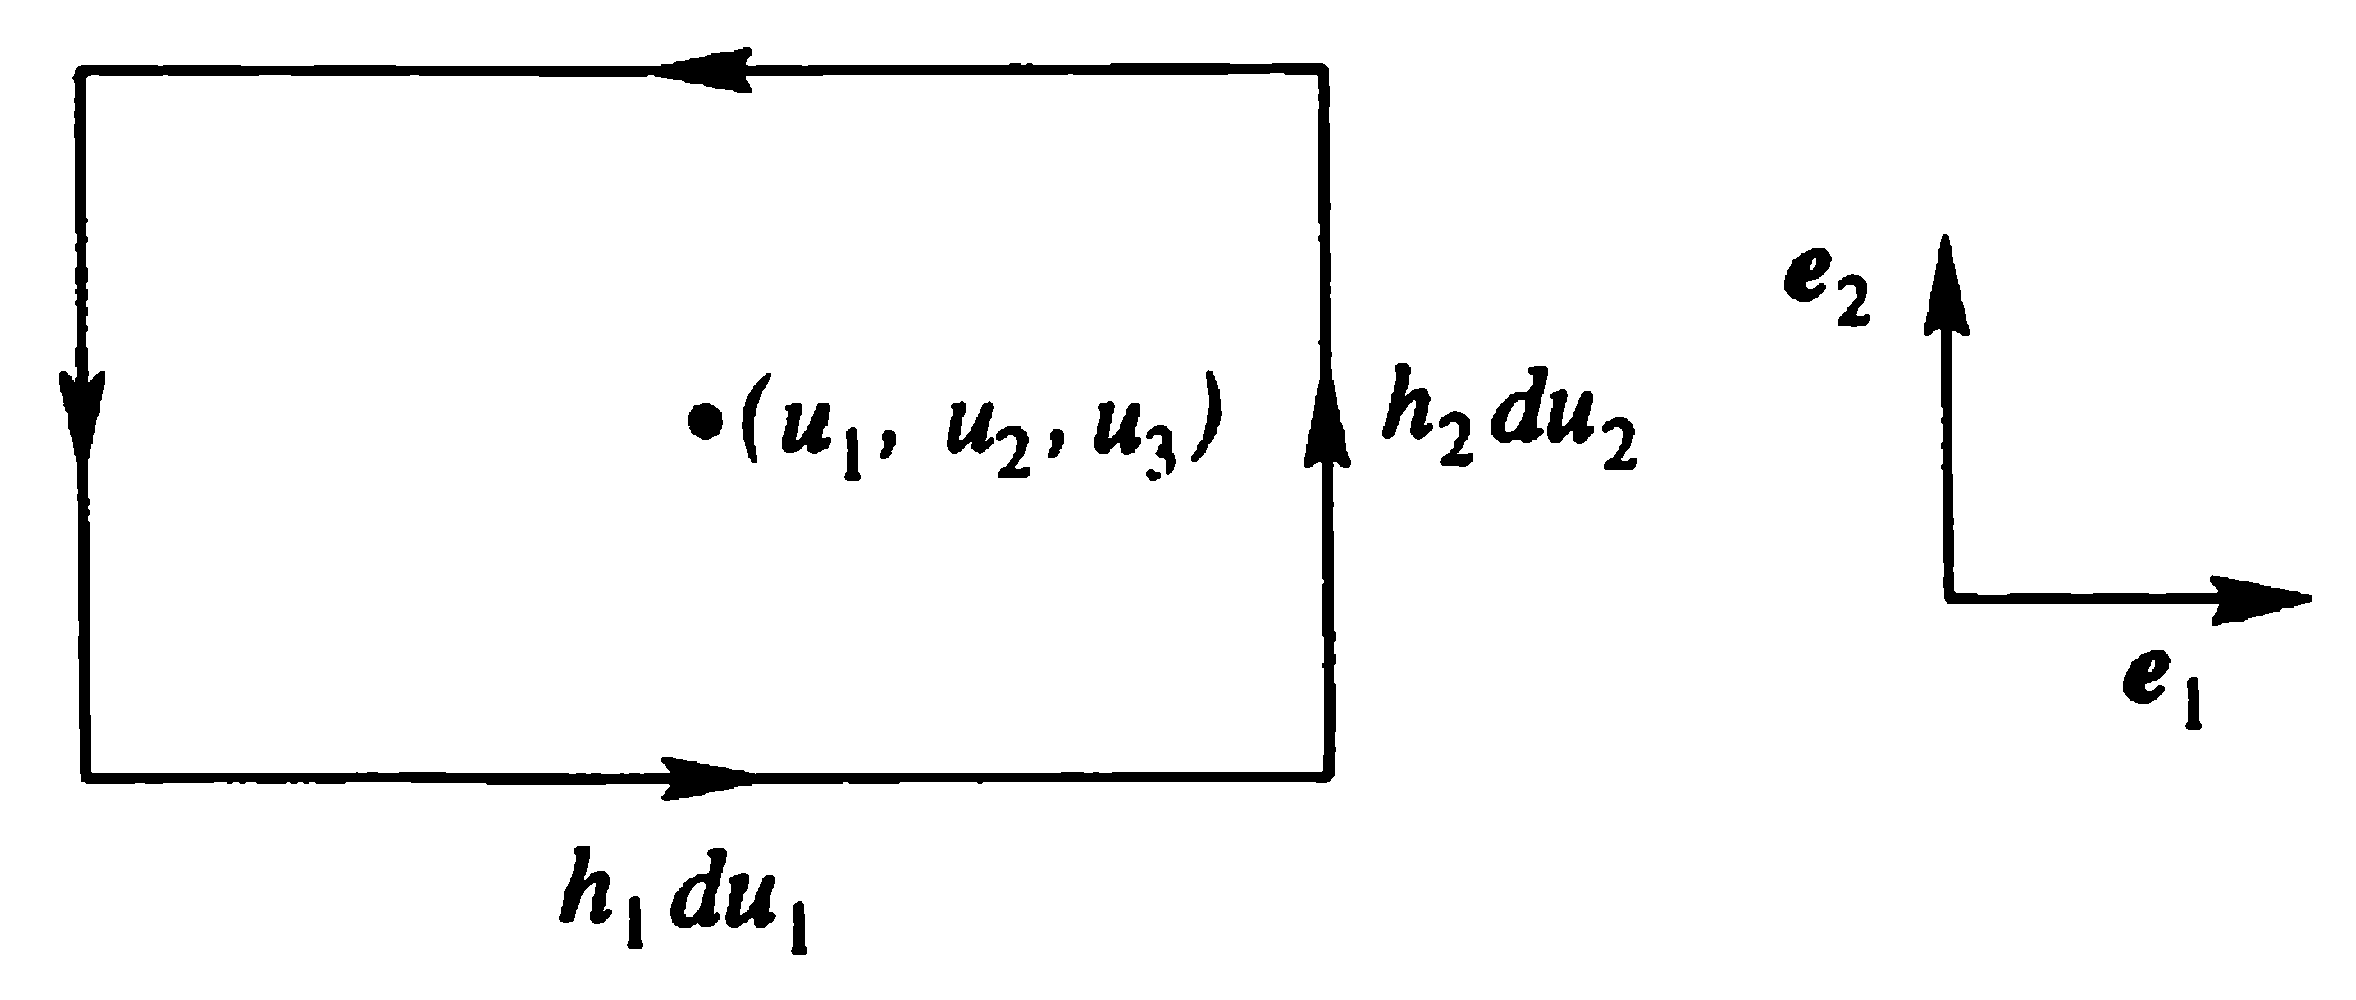
\includegraphics[scale=0.3]{fig/a-3.eps}
    \caption{计算旋度}
\end{figure}
\begin{figure}[htbp]
    \centering
    \label{曲线坐标微元}
    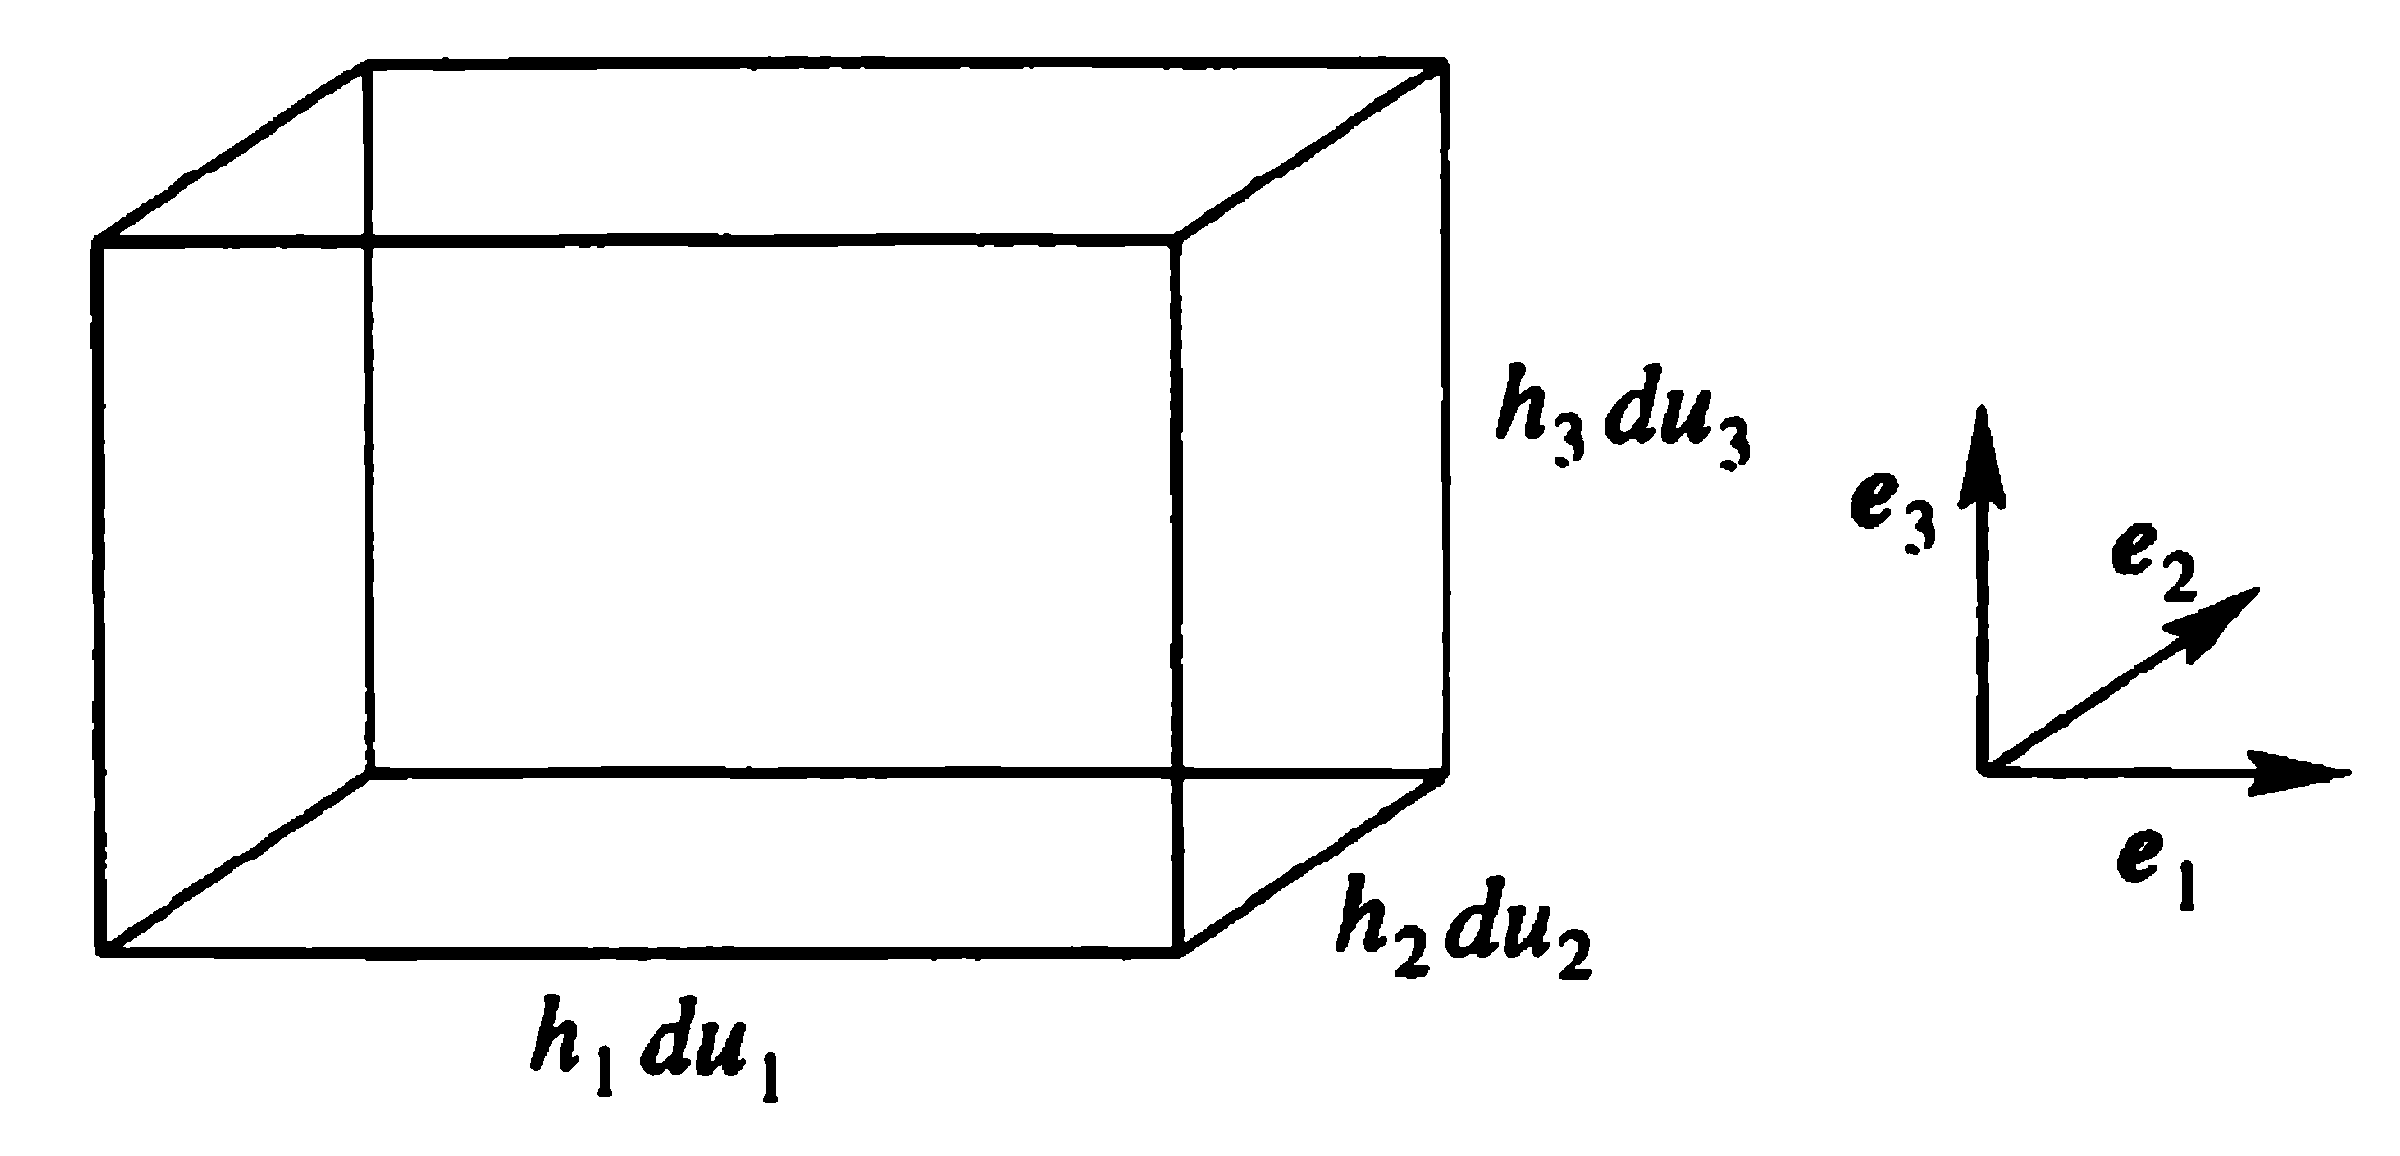
\includegraphics[scale=0.26]{fig/a-2.eps}
    \caption{曲线坐标系的局部就可以看成一个小(不再是直角坐标里面的正方体了), 图中也标出了参数微元和实际位移量的比例关系}
\end{figure}
\section{直角坐标里的张量}
\chapter{Linear Algebra}


\end{document}